\documentclass{standalone}
\usepackage{tikz}

\begin{document}

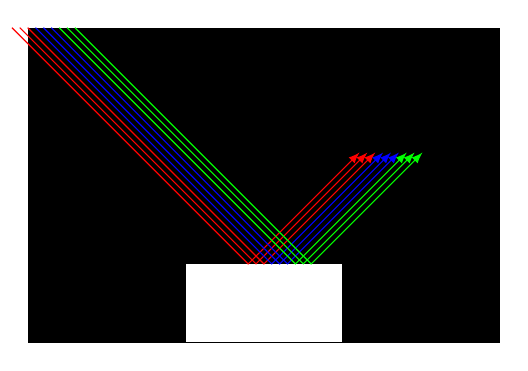
\begin{tikzpicture}
  \path[fill=black,use as bounding box] (-3,-1) rectangle (3,3);
  \draw[fill=white] (-1,-1) rectangle (1,0);

  \draw[red,-latex] (-3,3) -- (0,0) -- ++(45:2);
  \draw[red,-latex] (-3.1,3) -- (-0.1,0) -- ++(45:2);
  \draw[red,-latex] (-3.2,3) -- (-0.2,0) -- ++(45:2);
  \draw[blue,-latex] (-2.9,3) -- (0.1,0) -- ++(45:2);
  \draw[blue,-latex] (-2.8,3) -- (0.2,0) -- ++(45:2);
  \draw[blue,-latex] (-2.7,3) -- (0.3,0) -- ++(45:2);
  \draw[green,-latex] (-2.6,3) -- (0.4,0) -- ++(45:2);
  \draw[green,-latex] (-2.5,3) -- (0.5,0) -- ++(45:2);
  \draw[green,-latex] (-2.4,3) -- (0.6,0) -- ++(45:2);
\end{tikzpicture}

\end{document}